% reports/01-k8s-maintainers/talk.tex
% Compile: pdflatex reports/01-k8s-maintainers/talk.tex   (run twice for frame numbers)
% Requires lstlean.tex installed globally (same setup as 00-checkpoint/talk.tex).
\documentclass[10pt,aspectratio=169]{beamer}

\usepackage[T1]{fontenc}
\usepackage[utf8]{inputenc}
\usepackage{amssymb}
\usepackage{upgreek}
\usepackage{color}
\usepackage{booktabs}

% lstlean.tex expects these named colors to be defined.
\definecolor{keywordcolor}{rgb}{0.7, 0.1, 0.1}
\definecolor{tacticcolor}{rgb}{0.0, 0.1, 0.6}
\definecolor{commentcolor}{rgb}{0.4, 0.4, 0.4}
\definecolor{symbolcolor}{rgb}{0.0, 0.1, 0.6}
\definecolor{sortcolor}{rgb}{0.1, 0.5, 0.1}
\definecolor{attributecolor}{rgb}{0.7, 0.1, 0.1}
\definecolor{errorcolor}{rgb}{1, 0, 0}
\definecolor{stringcolor}{rgb}{0.5, 0.3, 0.2}

\usepackage{listings}
\def\lstlanguagefiles{lstlean.tex}
\lstset{language=lean}

\usepackage{tikz}
\usetikzlibrary{arrows.meta, positioning, calc, fit, backgrounds}

% ---- minimal beamer styling -------------------------------------------------
\usetheme{default}
\setbeamertemplate{navigation symbols}{}
\setbeamertemplate{footline}[frame number]
\setbeamerfont{frametitle}{size=\large,series=\bfseries}
\setbeamercolor{frametitle}{fg=black}
\setbeamercolor{structure}{fg=black!75}
\setbeamertemplate{itemize item}{\textbullet}

\hypersetup{colorlinks=true, urlcolor=blue!60!black, linkcolor=blue!60!black}

\lstset{
  basicstyle=\ttfamily\scriptsize,
  keywordstyle=\bfseries,
  commentstyle=\itshape\color{black!55},
  showstringspaces=false,
  columns=fullflexible,
  breaklines=true,
  xleftmargin=4pt,
  aboveskip=4pt, belowskip=4pt,
}

\tikzset{
  box/.style    ={draw, rounded corners=2pt, align=center,
                  minimum height=0.95cm, minimum width=2.6cm, font=\small},
  pill/.style   ={draw, dashed, rounded corners=2pt, align=center,
                  minimum height=0.7cm, font=\scriptsize, inner sep=3pt},
  arr/.style    ={-{Stealth[length=2.2mm]}, thick},
  lbl/.style    ={font=\scriptsize, inner sep=1pt},
  bad/.style    ={draw, rounded corners=2pt, align=center, fill=red!8,
                  minimum height=0.8cm, minimum width=2.4cm, font=\scriptsize},
  good/.style   ={draw, rounded corners=2pt, align=center, fill=green!8,
                  minimum height=0.8cm, minimum width=2.4cm, font=\scriptsize},
}

\title{\bfseries Modeling Kubernetes invariants in Lean}
\author{Sachin Singh}
\date{}

\begin{document}

% ============================================================================
% 1. TITLE
% ============================================================================
\begin{frame}
  \titlepage
  \vspace{-0.6em}
  \centerline{\small\url{https://github.com/sachinkumarsingh092/lean-rl/tree/master/lean_rl/lean}}
\end{frame}

% ============================================================================
% 2. COLD OPEN
% ============================================================================
\begin{frame}{A routine scale-down}
\large
\begin{center}
\texttt{\$ kubectl scale deploy/web {-}{-}replicas=1}
\end{center}
\vspace{0.6em}
\small
\begin{itemize}\itemsep0.35em
  \item The webhook admits it and the deployment scales down.
  \item \texttt{web} had a PDB with \texttt{minAvailable: 2}.
  \item The PDB controller logs the violation, but only after the cluster has already lost the guarantee.
  \item Customers see the blip and the pager fires.
\end{itemize}
\vspace{0.6em}
\centerline{\itshape The thing that's missing is a model of what the cluster will look like next.}
\end{frame}



% ============================================================================
% 3. WHY THIS KEEPS HAPPENING
% ============================================================================
\begin{frame}{Why this keeps happening}
\begin{itemize}\itemsep0.5em
  \item Validating webhooks evaluate the \textbf{incoming object}, not the \textbf{post-state of the cluster}.
  \item Cluster-wide invariants are enforced by \textbf{controllers, after the write lands}:
  \begin{itemize}\itemsep0.15em
    \item PDB \texttt{minAvailable}
    \item node CPU and memory capacity
    \item anti-affinity and topology spread
    \item ResourceQuota
  \end{itemize}
  \item That is reconciliation, not prevention. It works eventually, but your SLO does not get to wait that long.
\end{itemize}
\end{frame}

% ============================================================================
% 2b. WHAT LEAN IS, BRIEFLY
% ============================================================================
\begin{frame}{What is Lean}
\begin{itemize}\itemsep0.5em
  \item Lean is a functional programming language whose compiler is also a proof checker.
  \item You write ordinary definitions: data structures, functions, predicates.
  \item You can also state theorems about those definitions and have the compiler check the proof.
  \item Same language, same file. The thing you prove about is the thing that runs.
  \item No model checker, no separate spec language. Just code, plus a proof obligation.
\end{itemize}
\end{frame}

% ============================================================================
% 4. TIMELINE: TODAY VS WITH GATE
% ============================================================================
\begin{frame}{Today vs.\ what we want}
\centering
\resizebox{0.95\textwidth}{!}{%
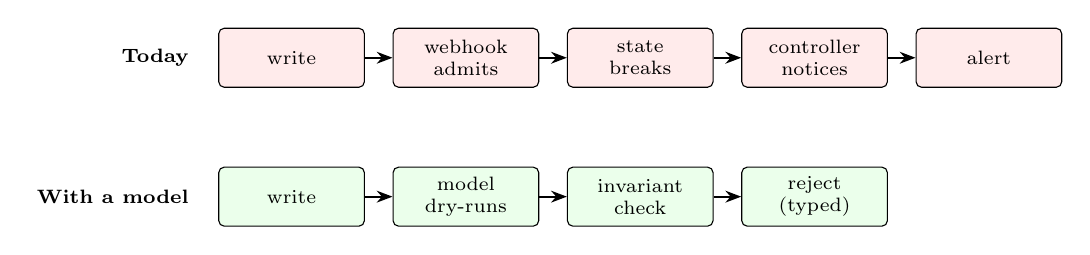
\begin{tikzpicture}[
    node distance=0.35cm and 0.35cm,
    bad/.style ={draw, rounded corners=2pt, align=center, fill=red!8,
                 minimum height=0.75cm, minimum width=1.85cm, font=\scriptsize,
                 inner sep=2pt},
    good/.style={draw, rounded corners=2pt, align=center, fill=green!8,
                 minimum height=0.75cm, minimum width=1.85cm, font=\scriptsize,
                 inner sep=2pt},
    arr/.style ={-{Stealth[length=2mm]}, thick},
  ]
  % Today
  \node[bad]                         (t1) {write};
  \node[bad, right=of t1]            (t2) {webhook\\admits};
  \node[bad, right=of t2]            (t3) {state\\breaks};
  \node[bad, right=of t3]            (t4) {controller\\notices};
  \node[bad, right=of t4]            (t5) {alert};
  \node[font=\scriptsize\bfseries, left=0.25cm of t1] {Today};
  \draw[arr] (t1)--(t2); \draw[arr] (t2)--(t3); \draw[arr] (t3)--(t4); \draw[arr] (t4)--(t5);

  % With a model
  \node[good, below=1.0cm of t1]     (g1) {write};
  \node[good, right=of g1]           (g2) {model\\dry-runs};
  \node[good, right=of g2]           (g3) {invariant\\check};
  \node[good, right=of g3]           (g4) {reject\\(typed)};
  \node[font=\scriptsize\bfseries, left=0.25cm of g1] {With a model};
  \draw[arr] (g1)--(g2); \draw[arr] (g2)--(g3); \draw[arr] (g3)--(g4);
\end{tikzpicture}}
\vspace{0.7em}\\
\centerline{\small The bad write never lands. The operator sees a structured reason instead of a postmortem.}
\end{frame}

% ============================================================================
% 5. THE PITCH IN ONE DIAGRAM
% ============================================================================
\begin{frame}{The model}
\centering
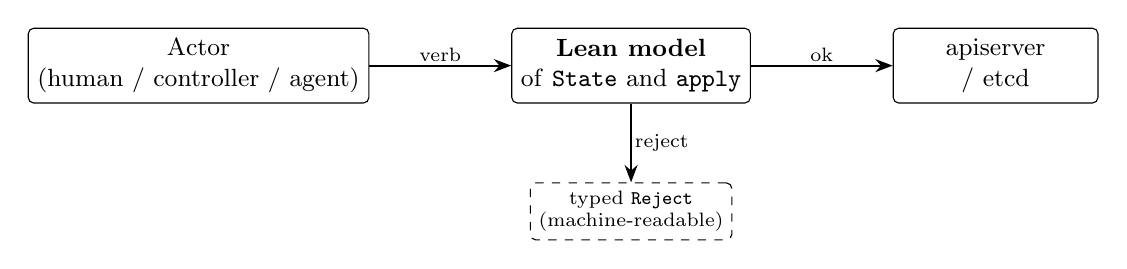
\begin{tikzpicture}[node distance=1.6cm and 1.8cm]
  \node[box]                       (actor) {Actor\\(human / controller / agent)};
  \node[box, right=of actor]       (gate)  {\bfseries Lean model\\of \texttt{State} and \texttt{apply}};
  \node[box, right=of gate]        (api)   {apiserver\\/ etcd};
  \node[pill, below=1.0cm of gate] (rej)   {typed \texttt{Reject}\\(machine-readable)};

  \draw[arr] (actor) -- node[lbl, above]{verb} (gate);
  \draw[arr] (gate)  -- node[lbl, above]{ok}   (api);
  \draw[arr] (gate)  -- node[lbl, right]{reject} (rej);
\end{tikzpicture}
\vspace{0.6em}
\begin{center}
\small\itshape
\texttt{apply : State $\to$ ApiVerb $\to$ State} is a function in Lean.\\
Once it is defined, post-state checks and proofs are just questions you can ask about it.
\end{center}
\end{frame}

% ============================================================================
% 6. ISN'T THIS GATEKEEPER / KYVERNO?  (early, on purpose)
% ============================================================================
\begin{frame}{``Isn't this Gatekeeper / Kyverno / CEL?''}
\small
\begin{tabular}{@{}lll@{}}
\toprule
                  & \textbf{Gatekeeper / Kyverno / CEL} & \textbf{Lean model} \\
\midrule
Evaluates         & Incoming object + cached refs       & Post-state $\mathit{apply}(s,v)$ \\
Coverage          & What the policy happens to check    & All states, all verbs \\
Backed by         & Reviewed policy code                & Kernel-checked theorem \\
\bottomrule
\end{tabular}
\vspace{0.8em}\\
\small
This is a different category. Gatekeeper and Kyverno are policy engines. What we have is a formal model of cluster transitions, which you can interrogate with a policy engine, an admission webhook, an RL judge, or a TLA+-style review.
\end{frame}


% ============================================================================
% 8. HOW IT WORKS -- 1: THE MODEL
% ============================================================================
\begin{frame}[fragile]{The model (1/3): state and verbs}
\begin{lstlisting}
structure State where
  pods        : List Pod
  nodes       : List Node
  deployments : List Deployment

inductive ApiVerb
  | createPod | createDeployment
  | updateDeployment | scaleDeployment | deletePodByKey

def apply : State → ApiVerb → State    -- pure, deterministic
\end{lstlisting}
\vspace{0.4em}
\small
This is a small slice of the API, expressed as plain data plus a single function. 
\end{frame}

% ============================================================================
% 9. HOW IT WORKS -- 2: INVARIANTS AS A REGISTRY
% ============================================================================
\begin{frame}[fragile]{The model (2/3): invariants are a registry}
\begin{lstlisting}
def invariants : List (InvariantKind × (State → Bool)) :=
  [ (.pdb,          pdbRespected),
    (.capacity,     capacityRespected),
    (.antiAffinity, antiAffinityRespected) ]

def safe (s : State) : Bool := invariants.all (·.2 s)
\end{lstlisting}
\vspace{0.4em}
\small
\begin{itemize}\itemsep0.2em
  \item Each invariant is just one decidable predicate on \texttt{State}.
  \item \textbf{Adding your own is one line in this list.}
  \item Topology spread, quota, and custom org-specific rules all have the same shape.
\end{itemize}
\end{frame}

% ============================================================================
% 10. HOW IT WORKS -- 3: THE GUARANTEE
% ============================================================================
\begin{frame}[fragile]{The model (3/3): what it lets us prove}
\begin{lstlisting}
theorem admitSafe :
    admit s v = .ok () → safe (apply s v) = true
\end{lstlisting}
\vspace{0.6em}
If \texttt{admit} returns \texttt{ok}, the resulting cluster state satisfies every registered invariant, for every state and every verb.
\vspace{0.6em}
\begin{itemize}\itemsep0.2em
  \item It is not ``the policy is correct because we reviewed it''.
  \item The Lean kernel checks the proof; we only have to write the invariant.
\end{itemize}
\end{frame}



% ============================================================================
% 13. BONUS: SAME GATE AS AN RL JUDGE
% ============================================================================
\begin{frame}{One use-case of the model: a judge for an LLM SRE agent}
\small
The same Lean definitions are also a useful referee when training an agent that proposes operations on a cluster.
\vspace{0.2em}
\begin{center}
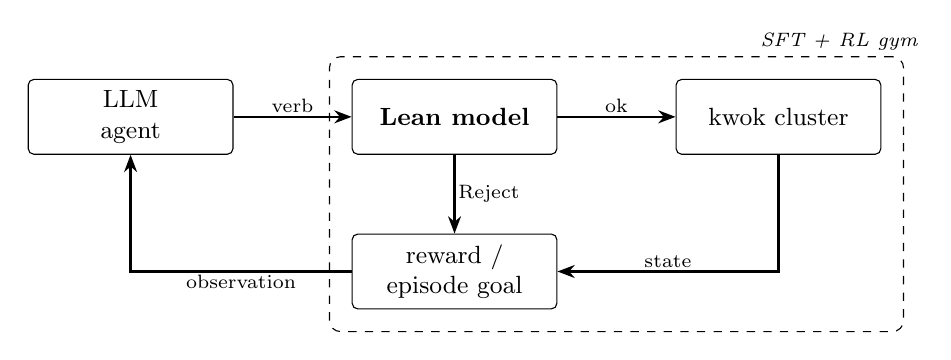
\begin{tikzpicture}[node distance=1.0cm and 1.5cm]
  \node[box]                       (llm)  {LLM\\agent};
  \node[box, right=of llm]         (lean) {\bfseries Lean model};
  \node[box, right=of lean]        (kwok) {kwok cluster};
  \node[box, below=1.0cm of lean]  (rwd)  {reward /\\episode goal};

  \draw[arr] (llm)  -- node[lbl, above]{verb} (lean);
  \draw[arr] (lean) -- node[lbl, above]{ok}   (kwok);
  \draw[arr] (lean) -- node[lbl, right]{Reject} (rwd);
  \draw[arr] (kwok) |- node[lbl, pos=0.75, above]{state} (rwd);
  \draw[arr] (rwd)  -| node[lbl, pos=0.25, below]{observation} (llm);

  \begin{scope}[on background layer]
    \node[draw, dashed, rounded corners=4pt, inner sep=8pt,
          fit=(lean)(kwok)(rwd),
          label={[font=\scriptsize\itshape, inner sep=2pt]
                 above right:SFT + RL gym}] {};
  \end{scope}
\end{tikzpicture}
\end{center}
\vspace{0.2em}
\footnotesize
\begin{itemize}\itemsep0.15em
  \item Typed \texttt{Reject} values become typed reward features. No regex on error strings.
  \item Decidable goals like \texttt{drainNode}, \texttt{rolloutImage}, and \texttt{scaleTo} give clean episode termination.
  \item Anything past \texttt{admit} is, by theorem, on a safe trajectory.
\end{itemize}
\end{frame}




% ============================================================================
% Open questions
% ============================================================================
\begin{frame}{Open questions}
\begin{itemize}\itemsep0.45em
  \item Is this slice of the API the right one to model first?
  \item Which cluster invariants are missing from the registry?
  \item Is the synchronous \texttt{apply} faithful enough, or do we need an explicit controller step?
  \item Where else would a formal model of the cluster pay off, beyond admission and agent training?
\end{itemize}
\end{frame}


\end{document}
